% Panel (a): Preprocessing — content only, no tikzpicture
% Uses spy library for zoom insets
% Origin is top-left of quadrant, content should fit within \panelW x \panelH

% === Raw image + spy inset ===
\begin{scope}[spy using outlines={
    rectangle, magnification=2.5, width=0.9cm, height=0.7cm,
    connect spies
  }]
  % Label above
  \node[font=\scriptsize\sffamily, text=stemgrey!80!black]
    at (0.30*\panelW, -0.22*\panelH) {Raw};
  % Image below label
  \node[inner sep=1pt, draw=stemgrey, thick]
    at (0.30*\panelW, -0.42*\panelH) (raw)
    {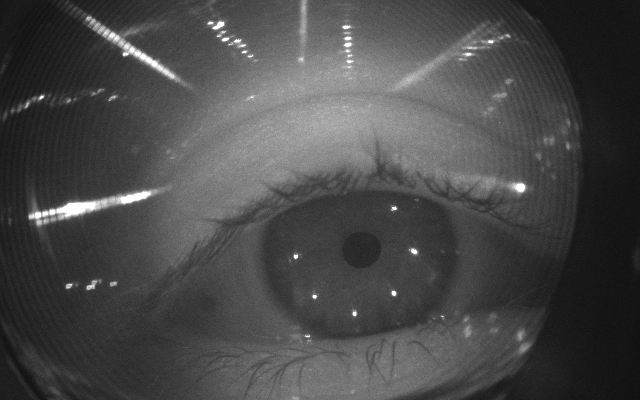
\includegraphics[width=1.5cm]{raw_eye.png}};
  % Inset: shifted up compared to before
  \spy[stemgrey!50,
    every spy in node/.style={draw=stemgrey!50, semithick},
    every spy on node/.style={draw=stemgrey!50, thin}]
    on ($(raw.center)+(0.05, -0.05)$)
    in node at ($(raw.south)+(-0.55, -0.25)$);
\end{scope}

% === Preprocessed image + spy inset ===
\begin{scope}[spy using outlines={
    rectangle, magnification=2.5, width=0.9cm, height=0.7cm,
    connect spies
  }]
  % Label above
  \node[font=\scriptsize\sffamily, text=stemgrey!80!black]
    at (0.70*\panelW, -0.22*\panelH) {Preprocessed};
  % Image below label
  \node[inner sep=1pt, draw=stemgrey, thick]
    at (0.70*\panelW, -0.42*\panelH) (preproc)
    {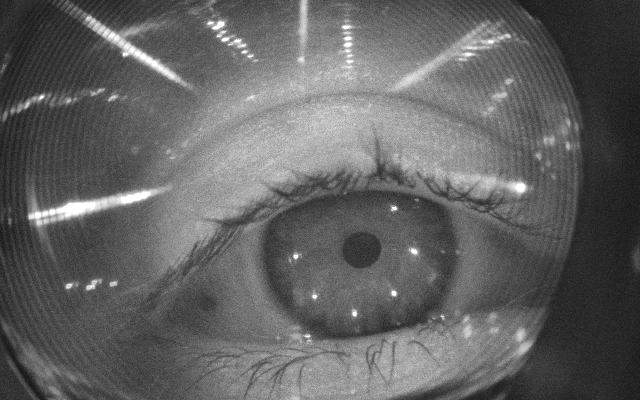
\includegraphics[width=1.5cm]{preprocessed_eye.png}};
  % Inset
  \spy[segteal!50,
    every spy in node/.style={draw=segteal!50, semithick},
    every spy on node/.style={draw=segteal!50, thin}]
    on ($(preproc.center)+(0.05, -0.05)$)
    in node at ($(preproc.south)+(-0.55, -0.25)$);
\end{scope}

% Arrow between main images
\draw[arr] (raw.east) -- (preproc.west);
